%SourceDoc ../YourName-Dissertation.tex
\chapter{Introduction -- Urban Computing} \label{chapter1:introduction}





\section{Model Region Interactions Incurred By Social Flow}


In the urban space, the movement of human population connects two disjoint regions, and brings influence from one to the other. \emph{My research focus is to capture the complicated interactions in the urban space with human mobility data}. 

In recent years, there are some large datasets of urban taxi going public~\cite{} under the FOIL\footnote{Freedom of information request law.}  The taxi data usually contains the pickup/drop-off time and location of one trip. By aggregating the taxi data, we are able to get the social flow among different regions.
Social flow data (e.g., commuting flow, taxi trajectories) are sensitive resources that urban planners can use to address city issues. 


Consider the following two examples. These two examples show that considering interactions of regions is an important problem to answer.


\textbf{Example 1.} \emph{Policy makers are deciding where to construct a shelter for families that are victims of violence. They understand the value of locating the shelter geographically far from violent neighborhoods. One possible choice is to locate the shelter in a neighborhood that is 10 miles from the violent neighborhoods where vulnerable families previously lived. However, a deeper analysis may reveal that the new neighborhood, though geographically removed from the old neighborhood, may still have strong social flows (connections caused by commutes, family visits) with the old neighborhood. Emerging research suggests that a great deal of crime happens in areas that are socially connected to offenders' neighborhoods. This suggests that shelters may benefit from being located in a neighborhood that is also socially isolated from violence (e.g., with weak communication and commuting interactions with the violent neighborhoods that shelter residents fled from) while socially connected to jobs, services, and resources.}


\textbf{Example 2.} \emph{\textcolor{red}{Find another example. The smart route selection scenario does not stand, since google map provides real time feedback on traffic jam. No need to infer}}





\section{Research Problems}


In the urban space, a model of region \textbf{interactions} bring solutions to the several fundamental data mining questions. We propose to view the city as a spatial network of communities linked by ``hyperlink'' flow. The questions we can answer are
\begin{itemize}
\item Understand nodes using links. Estimate an unobserved property of focal community, given the observations on other communities and other types of data. For example, the crime rate in a residential neighborhood could be impacted by  non-adjacent but flow-connected neighborhoods, because the residents in the neighborhoods are also exposed to and influenced by the environment in the workplace.
\item Understand links using nodes. Are certain properties of two connected nodes associated with the type and volume of the flow connections? For example, given the crime profiles of two connected communities, which type of interactions (taxi, LEHD, or space continuity) is more important in forming the crime properties?
\item Identify the fundamental dependency structure among properties of nodes. For example, the crime rate of two connected communities may show a strong correlation. However, this does not necessarily mean that high crime rate in one community lead to the high crime in another. The crime is very likely to be caused by other properties. 
\end{itemize}




\section{Existing Work}



Traditionally, most urban research  do not use flow data, since the data is not available. For example, researchers have used demographic information (e.g., population poverty level, socioeconomic disadvantage, racial composition of population) to estimate the crime rate in a community~\cite{GrSa09}. However,  such demographic information only contains partial information about the neighborhoods and does not dynamically reflect the changes in the community. Using only demographic information will result in a relative error of at least 30\% for crime rate estimation in Chicago (refer to experiment section in the paper).



\textbf{Use spatial influence as interactions}.
Since there is no flow data available, spatial similarity is widely accepted assumption to model the region interactions. \textbf{Spatial similarity} assumes that spatially adjacent regions tend to have similar properties. In urban space, most data reflect the properties of human beings, such as the traffic volume, crime count, and geo-tagged tweets. Therefore, these data are attached to human crowd instead of a specific location. 
In the urban space, the intuition behind the \textbf{spatial similarity} is that human movement is regular, and most of our daily activities are conducted in a limited area.

There is one existing study using the geographical influence~\cite{Ans02} to estimate the crime rate, i.e., the crime in the nearby communities can be propagated to the focal community. But this geographical influence is of little help in improving the crime inference on top of demographic feature, with at most 0.4\% relative improvement in our experiments. This is probably because the nearby communities also share similar demographics, which limits the additional benefit of geographical influence. In the study, spatial autoregressive model is used

\begin{equation}
\label{eq:sar}
y = \rho_1 W^{spatial} y + X \beta + \epsilon,
\end{equation}
where $y$ is the crime count, $X$ is the demographics property, and $W^{spatial}$ is an $n\times n$ spatial distance matrix.



\textbf{Simple extension on spatial influence model}
It is easy to extend the spatial autoregressive model in Equation~\ref{eq:sar} with a social flow matrix.
\begin{equation}
\label{eq:sar2}
y = \rho_1 W^{spatial} y + \rho_2 W^{network} y + X \beta + \epsilon,
\end{equation}
where $W^{network}$ is an $n\times n$ social distance matrix.
It is clearly that the interaction term $\rho_2 W^{network} y$ is ad-hoc, since there could be other combinations like $\rho_3 W^{network} x_1$.





\section{Challenges}

The interactions usually take the the following form $m(f_{ij}, x_j)$.

\textbf{Given one type of social flow, define interaction is non-trivial}. Given only one type of social flow, there are too many possibilities in constructing interactions.   1) The flow matrix can take various form. For example, we can chose normalize it or not. When normalizing the flow matrix, we can chose whether normalize by in-flow or out-flow. 
2) There are also many nodal properties that could interact with their neighbors, such as various demographics features. 
3) Different kinds of function can be used to define interactions. Take the product of flow and nodal properties is the most straightforward choice. However, sometimes it also makes sense to further apply a distance exponential decay on previous product.
Therefore, the construction of interaction is totally ad-hoc. 


\textbf{Given multiple types of social flow, the interaction is more difficult to define}. It is possible we have multiple types of social flow (e.g. taxi flow, commuter transit). For one pair of regions, should we build separate interaction over different social flows, or sum over all flows to get one interaction? When we take the sum, should we weight different social flow differently, and how?


\textbf{The interaction could be spatial non-stationary}. Most models in existing work are global model, which assumes the statistic interaction does not vary over space. However, some urban data have spatial non-stationary property. Use Chicago crime as example, shown in Figure~\ref{fig:chi-crime}. It is clear that using global estimates of relationships can present misleading interpretations of local relationships.


\begin{figure}[h]
\centering
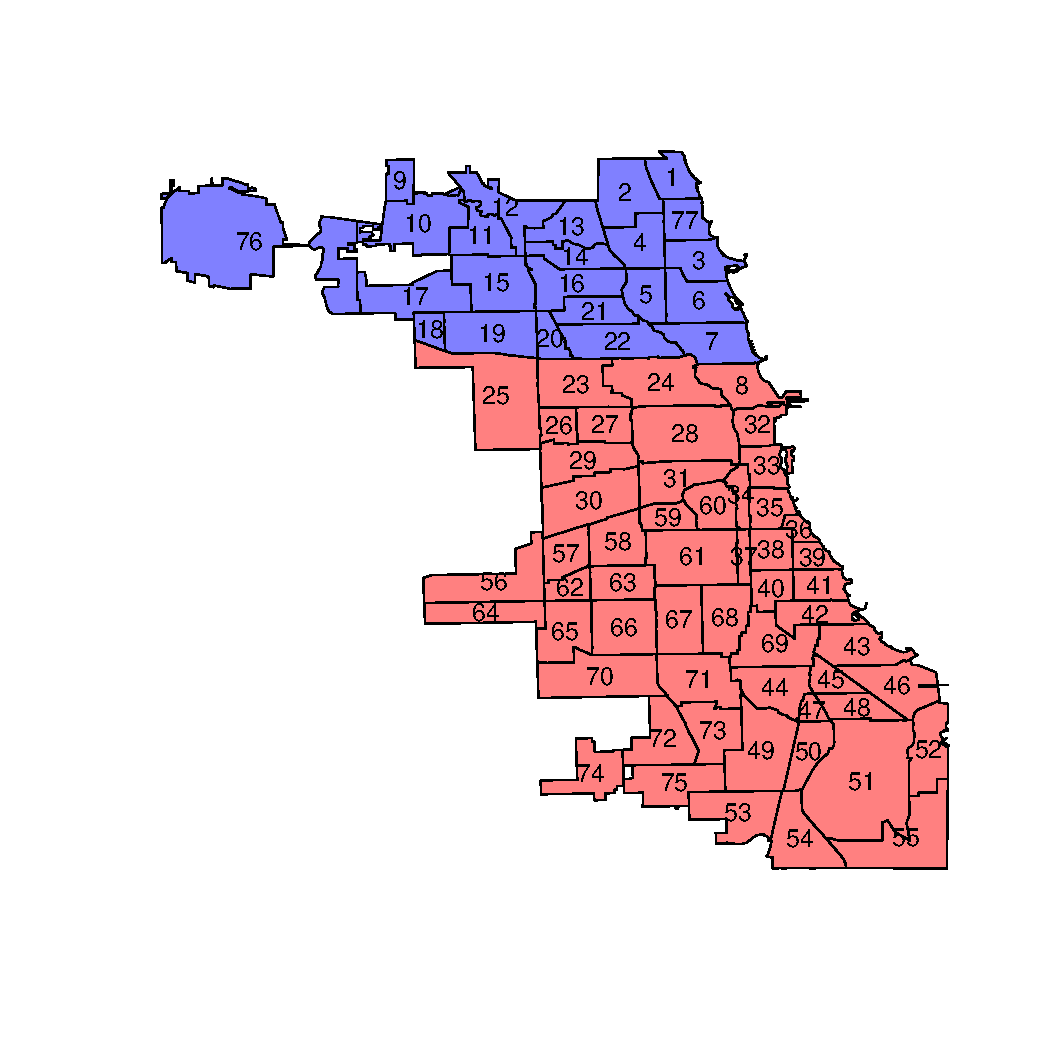
\includegraphics[width=0.45\textwidth]{fig/north-south-split.pdf}
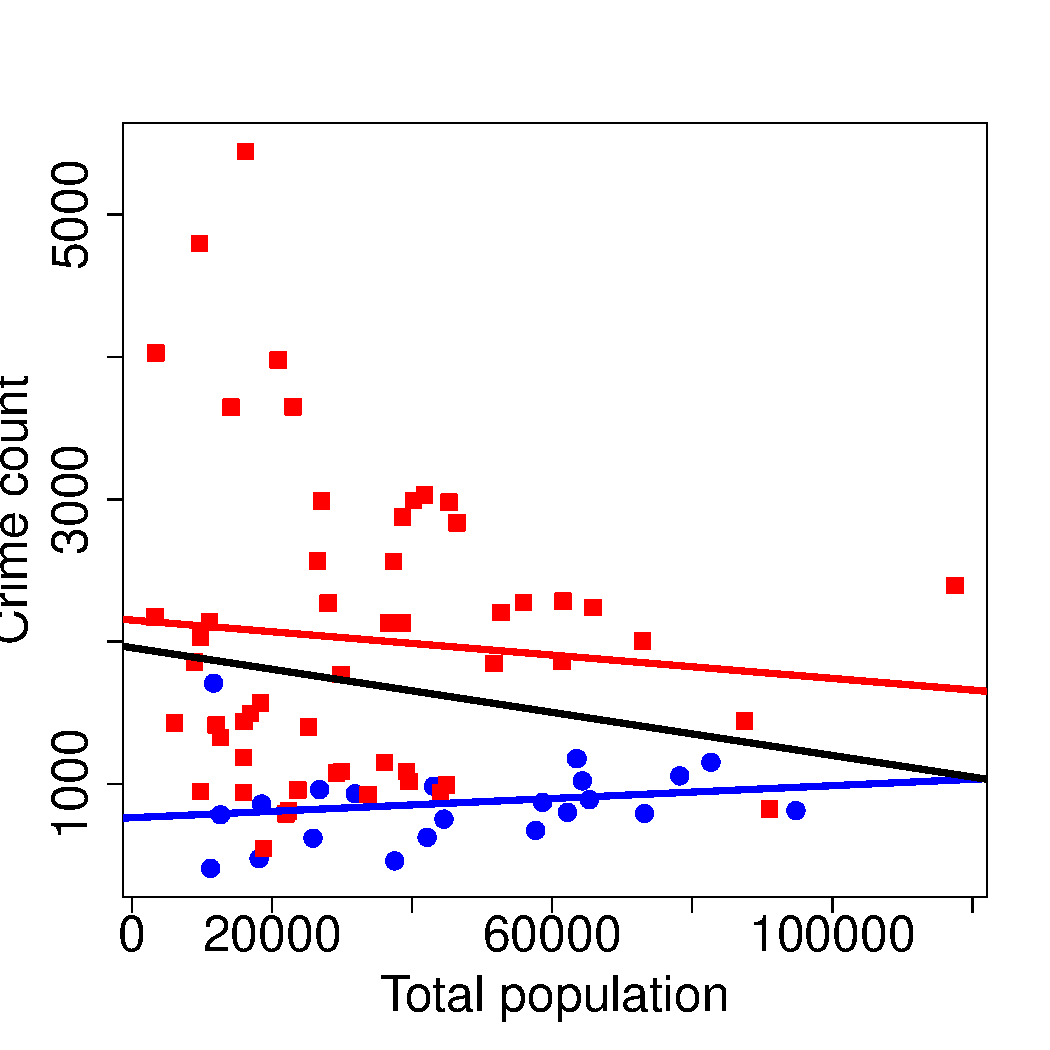
\includegraphics[width=0.45\textwidth]{fig/crime-pop.pdf}
\caption{The crime count vs. total population relationship shows spatial non-stationary property.}
\label{fig:chi-crime}
\end{figure}





\section{A Unified Graphical Model}

We propose a unified graphical model to capture the interactions among regions. Since various flow connect regions into various network. A graphical model is a natural way to represent the whole system. Additionally, this model can address the two drawbacks mentioned above.

To address the non-trivial definition of interaction. In the graphical model we model the interaction of two communities is a hidden variable. This hidden variable is connected with the observations on both flow and nodal properties. We can learn the interaction from the network.

To address the spatial non-stationarity. Each region is built as separate node in the graphical model. This way, the conditional probability 
\[ P(y_i | X_i) \]
is different at different regions, which is equivalent to have mutliple local models to capture the different relations between $y$ and $X$.





In next chapter we study the first problem - ``using links to understand nodes''. We use crime inference as an example, in which we use an enhanced spatial autoregressive model to predict crime count of a community using its neighbors. In Chapter \ref{ch:crf}. We first discuss the missing property of a spatial autoregressive model, which is the spatial non-stationarity. To address this, we propose a conditional random field based  graphical model. This model is superior than other method in the literature, such as geographically weighted regression. Finally, there is a research plan in Chapter \ref{ch:plan}.



